%%%%%%%%%%%%%%%%%%%%%%%%%%%%%%%%%%%%%%%%%%%%%%%%%%%%%%%%%%%%%%%%%%%%%%%%%%%
%
% Template for a LaTex article in English.
%
%%%%%%%%%%%%%%%%%%%%%%%%%%%%%%%%%%%%%%%%%%%%%%%%%%%%%%%%%%%%%%%%%%%%%%%%%%%

\documentclass{article}

% AMS packages:
\usepackage{amsmath, amsthm, amsfonts}
%%\usepackage{algorithm}
\usepackage[]{algorithm2e}
\usepackage[hyperref, UTF8]{ctex}
\usepackage[noend]{algpseudocode}
\usepackage{graphicx}
\usepackage{subcaption}
\usepackage[top=0.8in, bottom=0.8in, left=1in, right=1in]{geometry}
\graphicspath{ {images/} }

% Theorems
%-----------------------------------------------------------------
\newtheorem{thm}{Theorem}[section]
\newtheorem{cor}[thm]{Corollary}
\newtheorem{lem}[thm]{Lemma}
\newtheorem{prop}[thm]{Proposition}
\theoremstyle{definition}
\newtheorem{defn}[thm]{Definition}
\theoremstyle{remark}
\newtheorem{rem}[thm]{Remark}

\makeatletter
\def\BState{\State\hskip-\ALG@thistlm}
\makeatother
%\newcommand*{\rom}[1]{\expandafter\@slowromancap\romannumeral #1@}
\newcommand{\rom}[1]{\uppercase\expandafter{\romannumeral #1\relax}}
% Shortcuts.
% One can define new commands to shorten frequently used
% constructions. As an example, this defines the R and Z used
% for the real and integer numbers.
%-----------------------------------------------------------------
\def\RR{\mathbb{R}}
\def\ZZ{\mathbb{Z}}

% Similarly, one can define commands that take arguments. In this
% example we define a command for the absolute value.
% -----------------------------------------------------------------
\newcommand{\abs}[1]{\left\vert#1\right\vert}

% Operators
% New operators must defined as such to have them typeset
% correctly. As an example we define the Jacobian:
% -----------------------------------------------------------------
\DeclareMathOperator{\Jac}{Jac}

%-----------------------------------------------------------------
\title{Isotopic Approximation within a Tolerance Volume}
\author{wegatron\\
  %% \small Dept. Templates and Editors\\
  %% \small E12345\\
  %% \small Spain
}

\begin{document}
\maketitle

%% \abstract{Compiling Embedded\_thin\_shell progress}
\section{Bad 3d delaunay triangulation}
  \begin{figure}[h]
    \begin{subfigure}[b]{0.4\textwidth}
      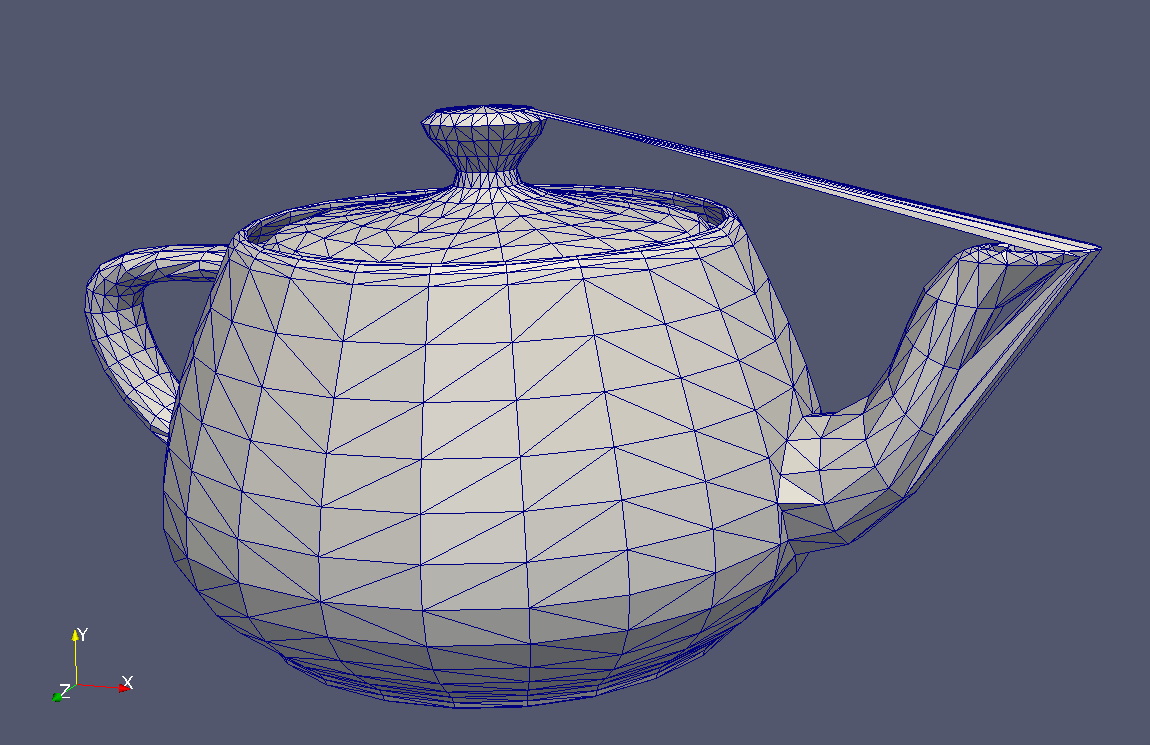
\includegraphics[width=\textwidth]{bad_surface0.png}
      \caption[现象]{bi+zero\_surface的四面体化}
    \end{subfigure}
    \begin{subfigure}[b]{0.4\textwidth}
      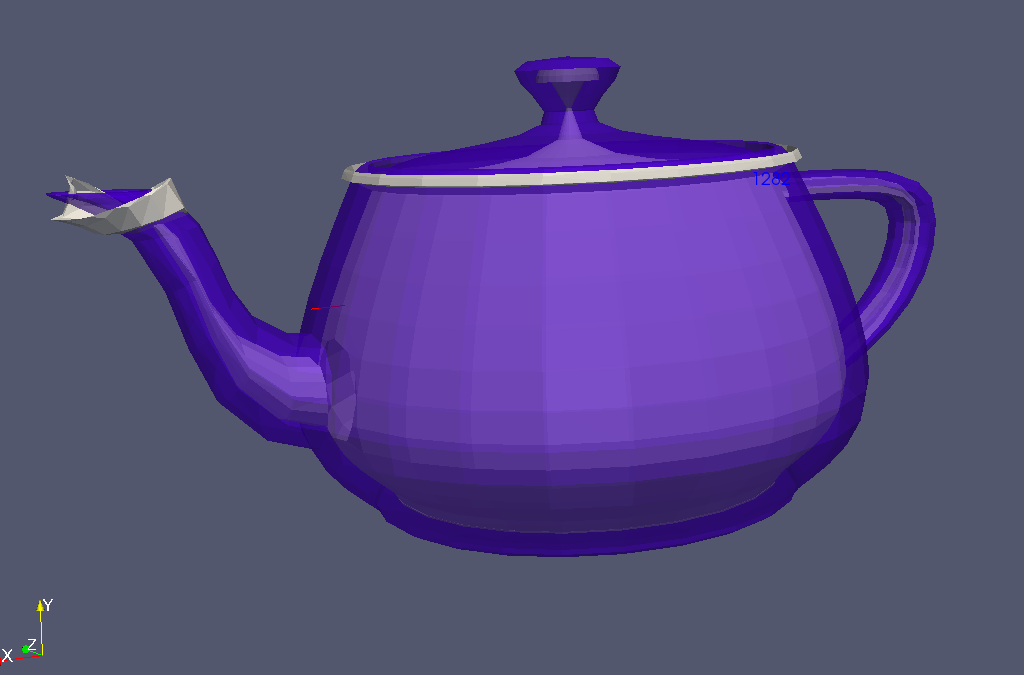
\includegraphics[width=\textwidth]{bad_surface1.png}
      \caption[原因]{zero\_surface和bi相交}
    \end{subfigure}
  \end{figure}

  \begin{figure}[h]
    \begin{subfigure}[b]{0.4\textwidth}
      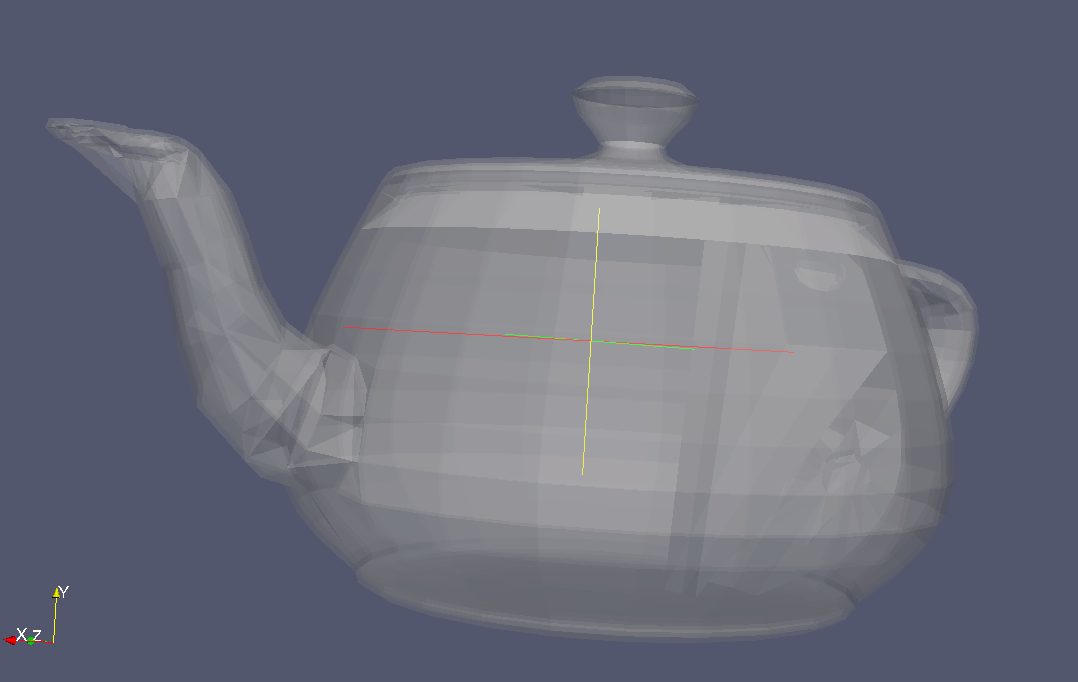
\includegraphics[width=\textwidth]{bad_inner_space0.png}
      \caption[现象]{bo+zero\_surface的四面体化}
    \end{subfigure}
    \begin{subfigure}[b]{0.4\textwidth}
      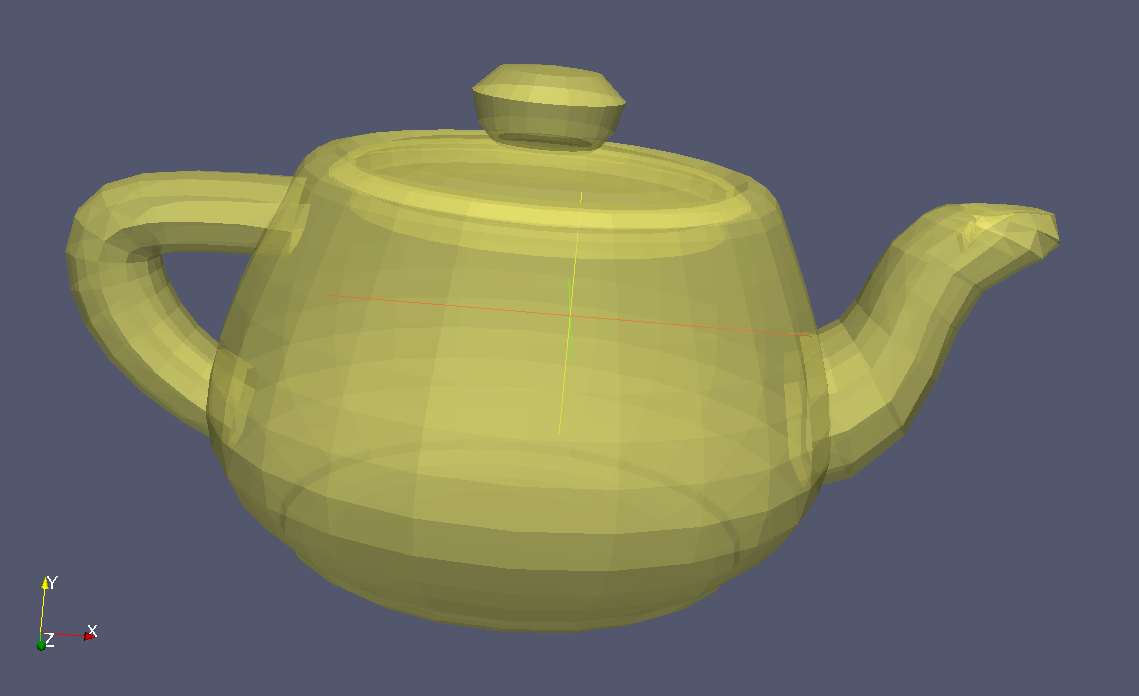
\includegraphics[width=\textwidth]{bad_inner_space1.png}
      \caption[原因]{bad inner space:teaport不连续,有洞}
    \end{subfigure}
  \end{figure}

  \section{Old Implementation}
  %% 理想情况下是:根据原模型(zero\_surface)做生成内外壳,并在保存内外壳的三角化的情况下做一个delaunay triangulation.
  %% 我原来的做法是:
  \begin{itemize}
  \item (bo+zero\_surface) + (bi+zero\_surface) 3D delaunay triangulation.
  \item Do edge collapse in zero\_surface.
  \end{itemize}
  problem: small number of edge collapsable number. Very large space to simlify.
  \section{Implementation steps}
  \begin{itemize}
    \item Do 3D delaunay triangulation with $p_{bi}+p_{bo}$, as the result of papers Refinement.
    \item Simplicial Tolerance:do edge collapse with bi-bi edges or bo-bo edges.
    \item Zero-set edge collapse.
    \item All edge edge collapse and then do Zero-set edge collapse again, if possible.
  \end{itemize}
  \subsection{Initial Triangulation}
  Do 3D delaunay triangulation with $p_{bi}+p_{bo}$, as the result of papers Refinement.
  And do sampling on the new surface of bi and bo, as the judge points. This result may not as good as the paper here.
  \begin{figure}[h]
    \begin{subfigure}[b]{0.5\textwidth}
        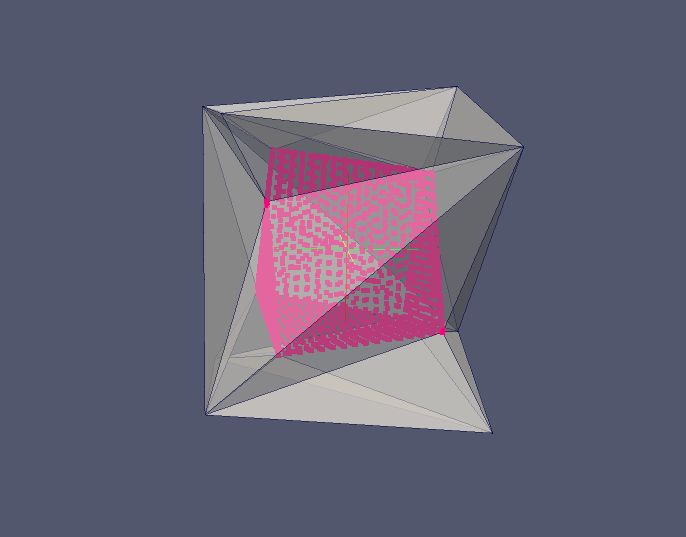
\includegraphics[width=\textwidth]{init_judge_points_0.png}
        \caption[a]{3d triangulation has no bo surface}
    \end{subfigure}
    \begin{subfigure}[b]{0.5\textwidth}
        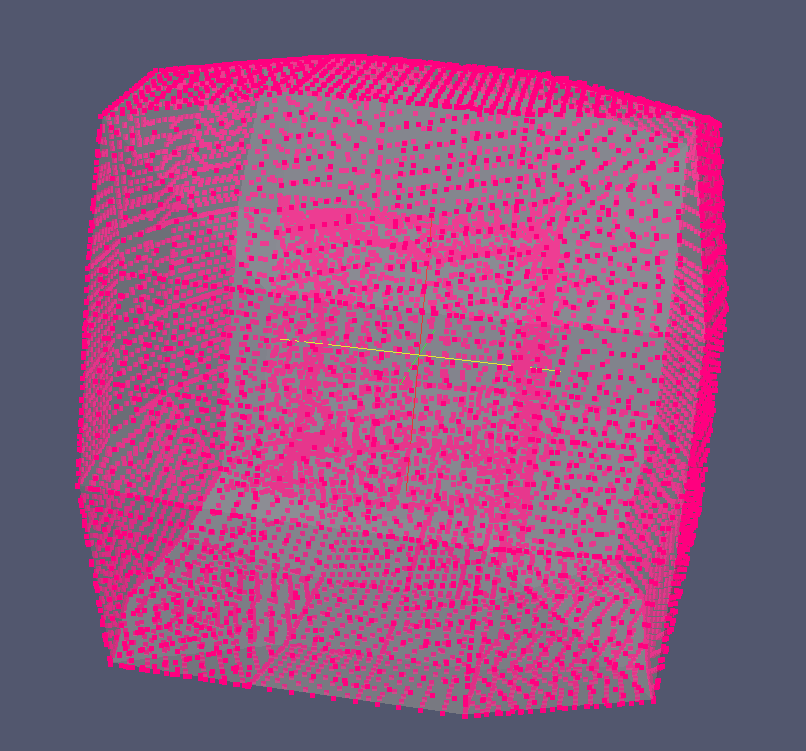
\includegraphics[width=\textwidth]{init_judge_points_1.png}
        \caption[a]{after subdivision.}
    \end{subfigure}
    \caption{The best way may be constrained delaunay triangulation.}
  \end{figure}
  \subsection{Simplicial Tolerance}
  \begin{figure}[h]
    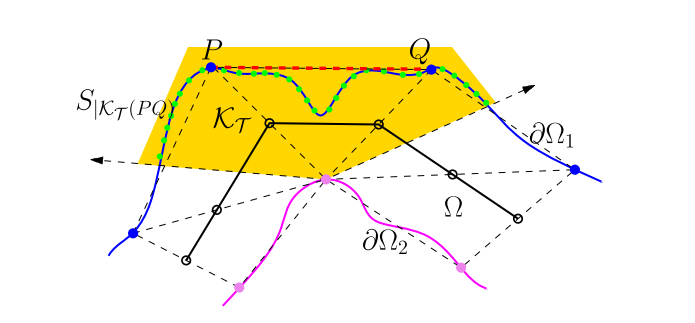
\includegraphics[width=\textwidth]{simplicial_tolerance.png}
    \caption{Do edge collapse with bi-bi edges or bo-bo edges, using the sample point as candicate.}
  \end{figure}
  The merge point choice by three condition:
  \begin{itemize}
    \item lay in the kernel region.
    \item do not leading to errors in the classification of S.
    \item the point with maximum error.
  \end{itemize}

  \begin{figure}[h]
      \begin{subfigure}[b]{0.5\textwidth}
        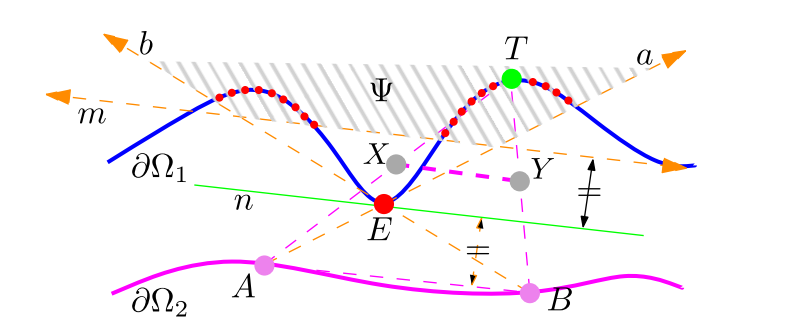
\includegraphics[width=\textwidth]{keep_classification0}
        \caption[a]{keep classification of S}
      \end{subfigure}
      \begin{subfigure}[b]{0.5\textwidth}
        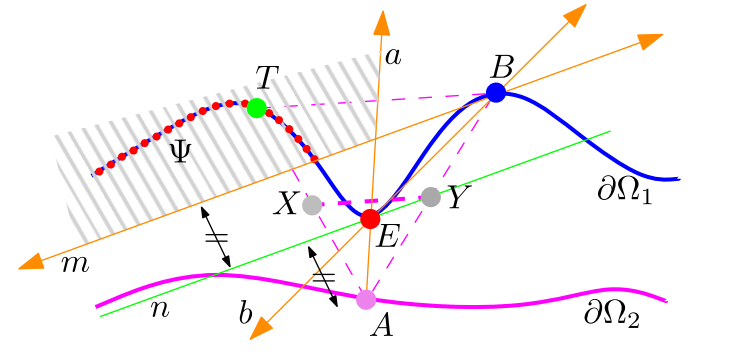
\includegraphics[width=\textwidth]{keep_classification1}
        \caption[b]{keep classification of S}
      \end{subfigure}
  \end{figure}

  \begin{algorithm}[H]
    \KwData{Tet mesh with sample point on bi and bo}
    \For{e $\in$ bo} {
      get all the sample points in its one-ring tets. all\_sp\_;\\
      get the points in kernel region. candi\_sp\_;\\
      \KwData{merge\_point, max\_error=-1}
      \For{each sample point $p \in candi\_sp\_$} {
        calculate all the sample point's error if edge collapse to p.\\
        \If{keep classification of S and error(p) $>$ max\_error} {
          merge\_point=p\\
          max\_error=error(p)
        }
      }
    }
   \caption{Simplicial tolerance}
\end{algorithm}
\end{document}
